\documentclass[10pt,twocolumn,letterpaper]{article}

\usepackage{cvpr}
\usepackage{times}
\usepackage{epsfig}
\usepackage{graphicx}
\usepackage{amsmath}
\usepackage{amssymb}

% Include other packages here, before hyperref.

% If you comment hyperref and then uncomment it, you should delete
% egpaper.aux before re-running latex.  (Or just hit 'q' on the first latex
% run, let it finish, and you should be clear).
\usepackage[breaklinks=true,bookmarks=false]{hyperref}

\cvprfinalcopy % *** Uncomment this line for the final submission

\def\cvprPaperID{****} % *** Enter the CVPR Paper ID here
\def\httilde{\mbox{\tt\raisebox{-.5ex}{\symbol{126}}}}

\newtheorem{definition}{\textit{Definition}}

\usepackage{siunitx}
% \usepackage[round-mode=places,round-precision=2,group-separator={,}]{siunitx}

% Pages are numbered in submission mode, and unnumbered in camera-ready
%\ifcvprfinal\pagestyle{empty}\fi
% \setcounter{page}{}
\begin{document}

%%%%%%%%% TITLE
\title{Translating Audio to MIDI\\ \vspace{0.1cm}\normalsize Fa Sol Fa Project -- Machine Learning for Vision and Multimedia}

\author{Paglialunga Federico\\
% Politecnico di Torino\\
% Corso Duca degli Abruzzi, Torino\\
{\tt\small s328876@studenti.polito.it}
% For a paper whose authors are all at the same institution,
% omit the following lines up until the closing ``}''.
% Additional authors and addresses can be added with ``\and'',
% just like the second author.
% To save space, use either the email address or home page, not both
\and
Risso Francesco\\
% Politecnico di Torino\\
% Corso Duca degli Abruzzi, Torino\\
{\tt\small s326834@studenti.polito.it}
\and
Tallone Samuele\\
% Politecnico di Torino\\
% Corso Duca degli Abruzzi, Torino\\
{\tt\small s334046@studenti.polito.it}
}

\maketitle
%\thispagestyle{empty}

%%%%%%%%% ABSTRACT
\begin{abstract}
Automatic Music Transcription (AMT) aims to convert raw audio into symbolic musical notation, typically in the form of MIDI. In this work, we present a convolutional neural network inspired by \textit{Spotify’s Basic Pitch} model, designed to transcribe piano recordings into MIDI sequences. Unlike the original implementation, which relies on specialized libraries, we re-implemented key components from scratch to maximize academic value and foster a deeper understanding of the underlying processes.
The model was trained and evaluated on the MAESTRO dataset, using constant-Q transforms and a custom data-loading pipeline. Our results demonstrate the viability of lightweight convolutional architectures for AMT and highlight trade-offs between optimized black-box approaches and transparent, educational implementations. 

\end{abstract}

%%%%%%%%% BODY TEXT
\section{Introduction}\label{sec:intro}
MIDI, or Musical Instrument Digital Interface, is a powerful data format because it captures the essence of musical performance in a structured, symbolic way.
Unlike audio, which records sound waves, MIDI encodes information like pitch, timing, velocity, and instrument type, making it highly editable and flexible.
This allows musicians and producers to tweak performances without any loss in quality, swap instruments instantly, and automate complex arrangements.

Converting a MIDI file to ``real'' audio is trivial, thanks to the use of audio fonts.
Creating directly a MIDI file from a live performance is also easy, as long as the instrument can provide such information. For instance, an electronic keyboard can directly output MIDI messages.
The most complex part is to go backwards, from a pre-recorded audio file to the corresponding MIDI.

Our project aimed to accomplish such task, in a controlled environment, where the audio is composed by a single instrument, a piano, playing some seconds of classical music.

For our model, we started from Spotify's Basic Pitch~\cite{spoty-audio} model description, to then adapt it to our needs.

\subsection{Paper structure}

This paper is structured as follows:
\begin{itemize}
    % \item Chapter \ref{sec:intro} describes the task, the paper structure and some background information about the MIDI protocol;
    \item \textbf{Chapter \ref{sec:background}} provides some background knowledge, such as the MIDI protocol and the CQT;
    \item \textbf{Chapter~\ref{sec:dataset}} illustrates the dataset that we used, as well as some preprocessing steps;
    \item \textbf{Chapter~\ref{sec:model}} analyzes the neural network model that we chose for the task, as well as the hyperparameters;
    \item \textbf{Chapter~\ref{sec:metrics}} provides descriptions for the metrics we used to evaluate the results;
    \item \textbf{Chapter~\ref{sec:experiments}} summarizes the different hyperparameter settings that we explored to find the best model;
    \item \textbf{Chapter~\ref{sec:conclusions}} describes the results we obtained;
    \item \textbf{Chapter~\ref{sec:future}} hints towards further improvements that could be made.
\end{itemize}

\section{Background}\label{sec:background}

\subsection{How MIDI works}

The MIDI protocol~\cite{midi-wiki} saves the music as a sequence of messages, each one describing an ``event'' created by the musician.
Each message contains at least two fields: the time elapsed since the previous event and the message type.
On top of that, each message type will hold all the necessary information to fully describe the event.
Some of the most common message types are:
\begin{itemize}
    \item Start of note. Includes information about which note is played (C4 has value \num{60}, then each semitone increases or decreases the value by \num{1}), and with how much strength it is played (from \num{0} to \num{127});
    \item End of note. Stores which note is not being played anymore;
    \item Control messages, that describe actions that alter the way the instrument sounds. They contain an identifier of the control (e.g. \num{4} for the foot pedal of the piano~\cite{midi-control}), and the corresponding value that is set.
\end{itemize}

\subsection{Constant-Q Transform}\label{ssec:CQT}

The Constant-Q Transform (CQT) is a mathematical signal processing tool that transforms a data series into the frequency domain. The calculation of the CQT follows these steps:
\begin{enumerate}
    \item consider the minimal frequency $f_0$ and the maximal frequency $f_{max}$ of the data, and choose the number of bins per octave $b$
    \item $K := \left\lceil b \cdot \log_{2}\!\left(\frac{f_{\max}}{f_0}\right) \right\rceil$
    \item $Q := \left( 2^{1/b} - 1 \right)^{-1}$
    \item for $k<K$ set $N_k := \left\lceil Q \frac{f_s}{f_k} \right\rceil$
    \item $x^{cq}[k] := \frac{1}{N_k} \sum_{n < N_k} x[n]\, w_{N_k}[n]\, e^{-2 \pi i n Q / N_k}$
\end{enumerate}

In our implementation, the \texttt{librosa} library is used to  automatically compute the CQT.

\subsection{Pitches, Notes and Onsets}

This section introduces key concepts that clarify the model’s outputs, with their meaning and implications.

\begin{definition}
    The \textbf{pitch} defines the rate of vibrations produced by a sound, that is, the degree of highness or lowness of a tone. We will indicate the tensor of pitches as $Y_p$.
\end{definition}

\begin{definition}
    The \textbf{onset} defines the beginning of the note at a given pitch. We will indicate the tensor of onsets as $Y_o$.
\end{definition}

\begin{definition}
    The \textbf{note} is a distinct and isolatable sound that acts as the most basic building block for nearly all of music. We will indicate the tensor of notes as $Y_n$.
\end{definition}

\begin{definition}
    The \textbf{posteriorgram} is a graph in which the x-axis is time and the y-axis contains distinct phonemes.
\end{definition}

We will represent the posteriorgrams of pitches, onsets and notes, in order to have the raw graphic images from which the MIDI file will be obtained.

\section{Dataset and Dataloader}\label{sec:dataset}
\subsection{Dataset}

For our training we used the MAESTRO~\cite{maestro} (MIDI and Audio Edited for Synchronous Tracks and Organization) dataset.
MAESTRO is a dataset of \num{1276} pieces of classical music played at the piano, each one saved both as audio and as MIDI.
In total, over \num{200} hours of music are available.
MAESTRO includes a suggestion for splitting its audios into training set (\num{962} recordings), validation set (\num{137}) and test set (\num{177}), which we followed.

\subsection{Dataloader}

As the Spotify team had done for Basic Pitch~\cite{spoty-audio}, we trained the model on portions of these audios, a random \num{2}-second sample for each training point.
This allowed on one side to reduce the computational time required, while at the same time it acted as a data augmentator: at each epoch, the model would see a different portion of the same audios, virtually removing the possibility of overfitting.

After a first examination, we noticed that the MIDIs only contained the piano track, while the audios also included other instruments, such as the violin.
Therefore, we decided to discard the original audios, and to create the inputs for the network by rendering the MIDIs ourselves.
This is either done once when the dataset is downloaded, or the audios can be generated on-the-fly just for the selected \num{2}-second portions.

Our dataloader additionally encodes the MIDI into a \texttt{numpy} array, to make it compatible with \texttt{torch}'s batching mechanism.

\section{Model}\label{sec:model}

The model has been built on the basis of the paper ``A Lightweight Instrument-Agnostic Model for Polyphonic Note Transcription and Multipitch Estimation''\cite{spoty-audio} for Spotify. Starting from the model structure given on the paper, we rebuilt the model using the \texttt{numpy} and \texttt{torch} libraries.

\subsection{Model structure}

We can divide the model structure into three parts:
\begin{itemize}
    \item \textbf{Preprocessing:} the input audio is transformed into the frequency domain;
    \item \textbf{Processing:} is the body of the model, composed by two branches of Conv2D series that estimate the correct posteriorgrams;
    \item \textbf{Postprocessing:} the obtained outputs from the processing stage are cleared and the MIDI file is created.  
\end{itemize}

\subsubsection{Preprocessing}

The model receives in input the audio, saved as a tensor, with a sample rate of $\num{22050}$ Hz and alongside a hop-size of $512$ samples. This translates to a duration of $23$ ms between consecutive frames.

Note that the sampling frequency chosen is half of the original audio sample rate. In this way, adequate content is preserved without unnecessary overhead. Indeed, the experiments confirmed that higher rates did not improve transcription quality.

The input is transformed into the frequency domain by means of CQT. The new tensor is further manipulated with a procedure of harmonic stacking: the harmonic frequencies of the original signal are partially overlapped and then summed.

These two steps compose the Harmonic Constant-Q Transform (HCQT).

\subsubsection{Processing}

The model is divided in two branches. Both the branches are full two-dimensional convolutional networks with ``same'' convolutions filtered by batch normalization, ReLU and/or sigmoid function.

The two branches then are concatenated and the output is given as input to one last ``valid'' Conv2D network. The complete scheme is visually summarized in figure\;\ref{fig:model-structure}.

The model has three outputs, which are time-frequency matrices, called posteriorgrams, encoding where a note is ``on'' ($Y_n$), where a pitch is active ($Y_p$) and the onset of that note ($Y_o$).

The architecture as, in total, $\num{21516}$ parameters.
% COMMENTINI: wonderful, love u 
% Ciau Fra <3

\subsubsection{Postprocessing}

The CNN produces in output the three posteriorgrams with $Y_p$, $Y_n$ and $Y_o$. They describe the input audio, with an image composed of continuous values.

The ideal tensor $Y_p$ has a binary nature, where the ``on'' values represent the actual notes to be inserted in the MIDI. To obtain a tensor of this format from the CNN output, a binarization step is performed, using a threshold that can be chosen manually by the user.

To create the midi, each pitch of each frame is checked to see if it's the start of a note. If so, the length of the note is computed, and the note is added to the MIDI.

A drawback of this implementation is that each note is always pressed with an arbitrary intensity, since from the outputs we do not have any information about how much ``loud'' the sound must be.

\begin{figure*}[ht]
    \begin{center}
        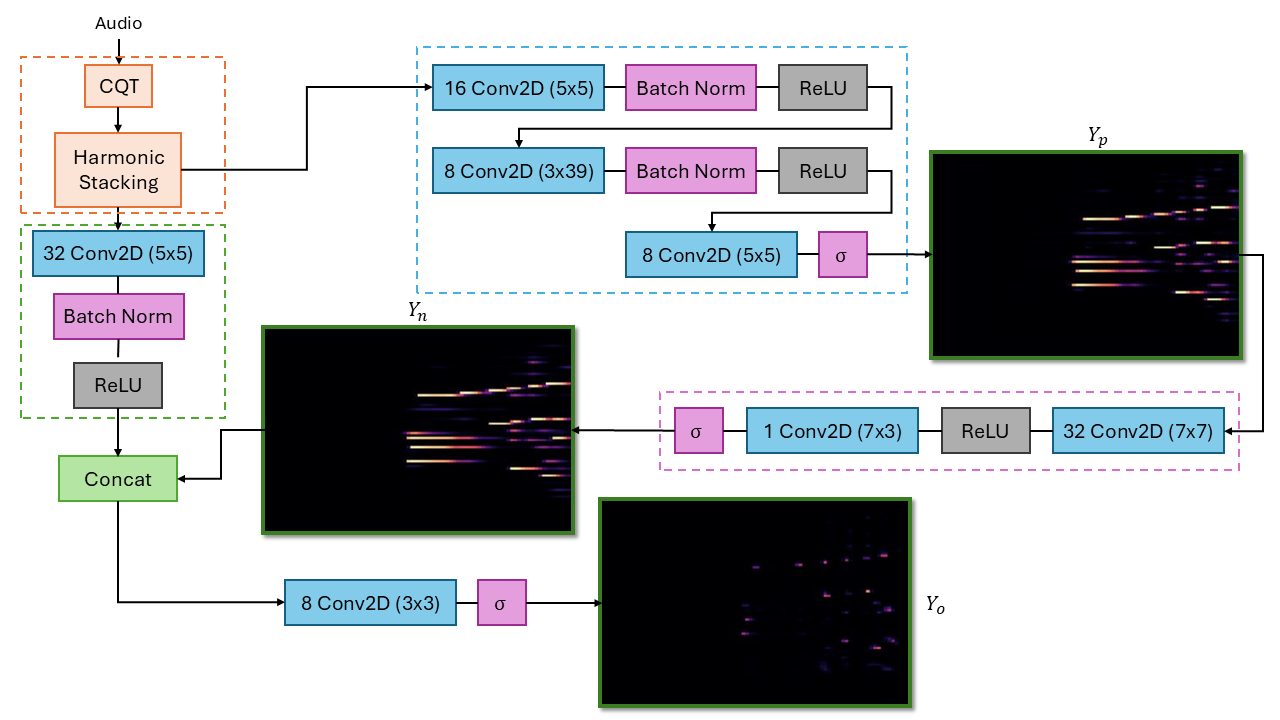
\includegraphics[width=0.9\textwidth]{"images/model-structure.png"}
    \end{center}
    \caption{Model structure representation}
    \label{fig:model-structure}
\end{figure*}

\subsection{Considerations on $Y_n$}

While other instruments, like the violin, can play the full spectrum of frequencies, the piano is restricted to a discrete set of keys. For this reason, the pitches' posteriorgram has to coincide with the notes' one.

Therefore, we also tried an alternative simplified model that does not consider the output $Y_n$, by directly concatenating $Y_p$. This option can be tried by setting the hyperparameter \texttt{remove\_yn = true}.

However, from the experiments we can see that better results are obtained by including the $Y_n$ in the model structure. Therefore, in this dissertation we will always consider the complete model.

\subsection{Hyperparameters}

All the hyperparameters can be managed in the \texttt{settings.py} file. The main hyperparameters we modified for the training are the following:

\begin{itemize}
    \item \textbf{learning rate};
    \item \textbf{weights on $Y_p$, $Y_o$, $Y_n$:} the Binary Cross Entropy (BCE) loss is a combination of the BCEs for the positive and negative ground truths. Since the ground truths include a much larger area which is silence, the negative BCE would be the main term. To balance it with the positive BCE, a weighted average is computed instead of the sum, using this weight as factor for the positive BCE;
    \item \textbf{weighted:} whether to take in consideration the previous weights or not;
    \item \textbf{label smoothing:} when set to $l$, the ground truth $G$ is replaced with $G{\cdot}(1-l)+0.5{\cdot}l$, to avoid the network being too confident, thus overfitting;
    \item \textbf{patience:} the number of consecutive epochs in which the evaluation loss is allowed not to improve, before stopping the training;
    \item \textbf{remove $Y_n$}.
\end{itemize}

The posteriorgram binarization threshold is not properly an hyperparameter, since it does not condition the training results.

Note that the number of epochs is also not a real hyperparameter, since we are using a patience mechanism: we only define it equal to a really high value that will never be reached. 

\section{Metrics}\label{sec:metrics}

\subsection{Loss formulation}

To evaluate the performance of the proposed model, we adopted the loss design introduced in the Spotify architecture~\cite{spoty-audio}, maintaining a multi-objective formulation.

Specifically, three distinct loss terms are computed, one for each output of the model (onset detection $Y_o$, pitch prediction $Y_p$, and note-level transcription $Y_n$), and subsequently summed to obtain the final optimization objective.

Each individual loss is implemented as a binary cross-entropy (BCE) function between the model predictions and the ground truth labels extracted from the corresponding MIDI files. In addition, we experimented with the application of label smoothing, which yielded a consistent improvement in performance.

\subsection{Class imbalance handling}

To address the inherent class imbalance of the dataset, arising from the predominance of silent frames compared to note events, we complemented the use of label smoothing with a weighting strategy that increases the contribution of positive samples within each output head. This approach enabled the network to better capture the relatively sparse note activations while reducing its bias towards predicting silence.

\subsection{Evaluation metrics}

To measure the performance of our adopted model we employed a combination of measures. 
We initially adopted the same test procedure followed in the Spotify model~\cite{spoty-audio}, measuring precision, recall and F1-score at the note level, utilizing specific tolerance windows. 
To be precise, a predicted note is considered correct when \textit{(i)} its onset is within \num{50} ms tolerance of the ground truth, \textit{(ii)} when its duration is within \num{20}\% tolerance of the reference length, and \textit{(iii)} the pitch is correct. 
While these metrics provide a good assessment of temporal alignment and duration consistency, their strictness is prone to yield quite low scores even for perceptually good transcription.

Apart from this, we also defined frame-level metrics that contrasted the estimated $Y_p$ piano-roll representation with the ground truth at the bin level, comparing the two posteriorgrams at the pixel level.

This enables us to capture in parallel two perspectives:
\textit{(i)} a note-level metric, that measures the number of unique individual notes that were labelled correctly based on the tolerance criteria, and 
\textit{(ii)} a bin-level metric, that measures how many of the time--frequency bins in the estimated piano-roll align with the ground-truth. 

\section{Experiments}\label{sec:experiments}

In this section, we analyze the behavior of out model by exploring how it was trained and the impact of various hyperparameter configurations on its output.

\subsection{Training}

Prior to full-scale training, we performed a sanity check to validate the model's learning capability. By training on a single data sample, we confirmed that the model could overfit and achieve near-perfect predictions, thus verifying that the implementation is functionally correct.

We also tested the model without the $Y_n$ branch, since with the piano the frequencies played always coincide with the notes, and we thought that having two outputs for the same information was redundant. However, testing showed that the results were very noisy and, therefore, even if the outputs are conceptually doing the same thing, we kept the branch because it improved the model’s performance.

Following this validation, we trained the model on the predefined MAESTRO~\cite{maestro} dataset split. We initialized it using hyperparameters similar to Spotify's~\cite{spoty-audio} final model architecture, this run acted as a performance baseline for all subsequent experimental runs. To be precise we used the following parameters: $Y_n = Y_p = \num{0.5}$, $Y_o = \num{0.9}$ weights, label smoothing $= \num{0.0}$, learning rate $=\num{0.001}$ and Adam optimizer that we kept for all the following runs.

\subsubsection{Learning rate}

We began hyperparameter tuning with the learning rate. An increase by a factor of $\num{10}$ led to rapid initial progress, but the training loss quickly plateaued. The validation loss was also highly unstable, an indicator that the optimizer was failing to converge to a robust solution. Reducing the learning rate by a factor of $\num{10}$, however, produced stable and smooth training and validation loss curves. Yet, this stability came at the cost of drastically slower training time for a very limited increase in performance.

For these reasons, we chose to leave the learning rate as $\num{0.001}$ for the most part when training, so that we could experiment more with other hyperparameters and lower it only when we were closer to the final solution.

\subsection{Weights of model outputs and label smoothing}

The configuration of the loss function's weighting scheme and the label smoothing parameter were identified as the hyperparameters with the most pronounced effect on the model's predictions. The weighting coefficient for the offset target $Y_o$ was deliberately fixed at a high value. This was necessary due to the severe class imbalance inherent to offset detection.

Our empirical results indicated that a complete absence of label smoothing encouraged the model to produce an abundance of note predictions. This configuration yielded a high recall metric but was coupled with critically low precision. Although the resultant F1-score was not radically dissimilar from that of the final model, the perceptual quality of the transcription was substantially inferior.

A noticeable refinement in output clarity was achieved by attenuating the weights for $Y_o$ and $Y_n$ to values on the order of $\num{0.1}$. Under this configuration, the model continued to exhibit a slight bias towards over-prediction, but the overall musical output was subjectively less contaminated by false positives.

The most substantial advancement was precipitated by the introduction of a minimal quantity of label smoothing ($\alpha = \num{0.005}$). This regularization technique successfully mitigated the model's overconfidence, leading to a notable increase in its precision. It also allowed us to remove the weights for $Y_n$ and $Y_p$. A counterproductive effect was observed when the smoothing factor was increased beyond an optimal threshold, causing the model to become overly conservative and frequently omit valid notes. We therefore converged on an intermediate value that negotiated a compromise between these two failure modes.

\subsection{Early stopping}

The ideal number of training epochs varied significantly based on the hyperparameters used. To handle this automatically, we implemented an early stopping rule. This mechanism stops training if the validation accuracy does not improve over a set number of consecutive epochs, a value we refer to as the patience, because this means that the model is starting to overfit or simply is not learning any new useful information. After that, it saves the model that achieved the best validation loss.

We adjusted this patience value as the experiments progressed. We began with a value of $\num{5}$ during initial testing. As we honed in on more promising configurations, we increased it to $\num{10}$, giving the model more time to converge.

The choice to use relatively low patience values was also a practical one. With limited hardware and time available, shorter training runs allowed us to conduct a much broader range of experiments, which was essential for finding the best overall model.

\subsection{Final model results}

For the final model we decided to train it in a two step process in order to extract some more performance and to have more stable results.
The first run was trained using the following hyperparameters:
\begin{itemize}
    \itemsep 0em
    \item \textbf{Learning rate:} $\num{0.005}$;
    \item \textbf{Label smoothing:} $\num{0.001}$;
    \item \textbf{$Y_o$, $Y_n$, $Y_p$ weights:} $0.\num{9}$, $\num{0.5}$ and $\num{0.5}$ respectively;
    \item \textbf{Adam optimizer};
\end{itemize}

For the refinement training label smoothing and the learning rate were changed both to $\num{0.0005}$, while the other parameters remained the same.

Here we present some statistics:
\begin{table}[h]
\centering
\begin{tabular}{|c|c|c|c|}
\hline
& \textbf{Precision} & \textbf{Recall} & \textbf{F1-Score} \\ \hline
\textbf{Training Set} & $\num{0.2351}$ & $\num{0.2180}$ & $\num{0.2262}$ \\ \hline
\textbf{Validation Set} & $\num{0.2237}$ & $\num{0.2113}$ & $\num{0.2173}$ \\ \hline
\textbf{Test Set} & $\num{0.2456}$ & $\num{0.2094}$ & $\num{0.2260}$ \\ \hline
\end{tabular}
\caption{Note-level evaluation results.}
\label{tab:note_results}
\end{table}

\begin{table}[h]
\centering
\begin{tabular}{|c|c|c|c|}
\hline
& \textbf{Precision} & \textbf{Recall} & \textbf{F1-Score} \\ \hline
\textbf{Training Set} & $\num{0.7854}$ & $\num{0.4720}$ & $\num{0.5896}$ \\ \hline
\textbf{Validation Set} & $\num{0.7597}$ & $\num{0.4738}$ & $\num{0.5836}$ \\ \hline
\textbf{Test Set} & $\num{0.7879}$ & $\num{0.4266}$ & $\num{0.5535}$ \\ \hline
\end{tabular}
\caption{Bin-level evaluation results.}
\label{tab:bin_results}
\end{table}

Although the numerical results of this model are not remarkable, its perceived performance is great, especially when dealing with shorter audio samples.

All the training runs are available on our \textbf{\textit{Weights \&\;Biases}} account\;\cite{wandb-link}.

We also include two samples corresponding to a one of the best model predictions (Figure~\ref{fig:best}) and one of the worst (Figure~\ref{fig:worst}) respectively:

\begin{figure}[ht]
\begin{center}
  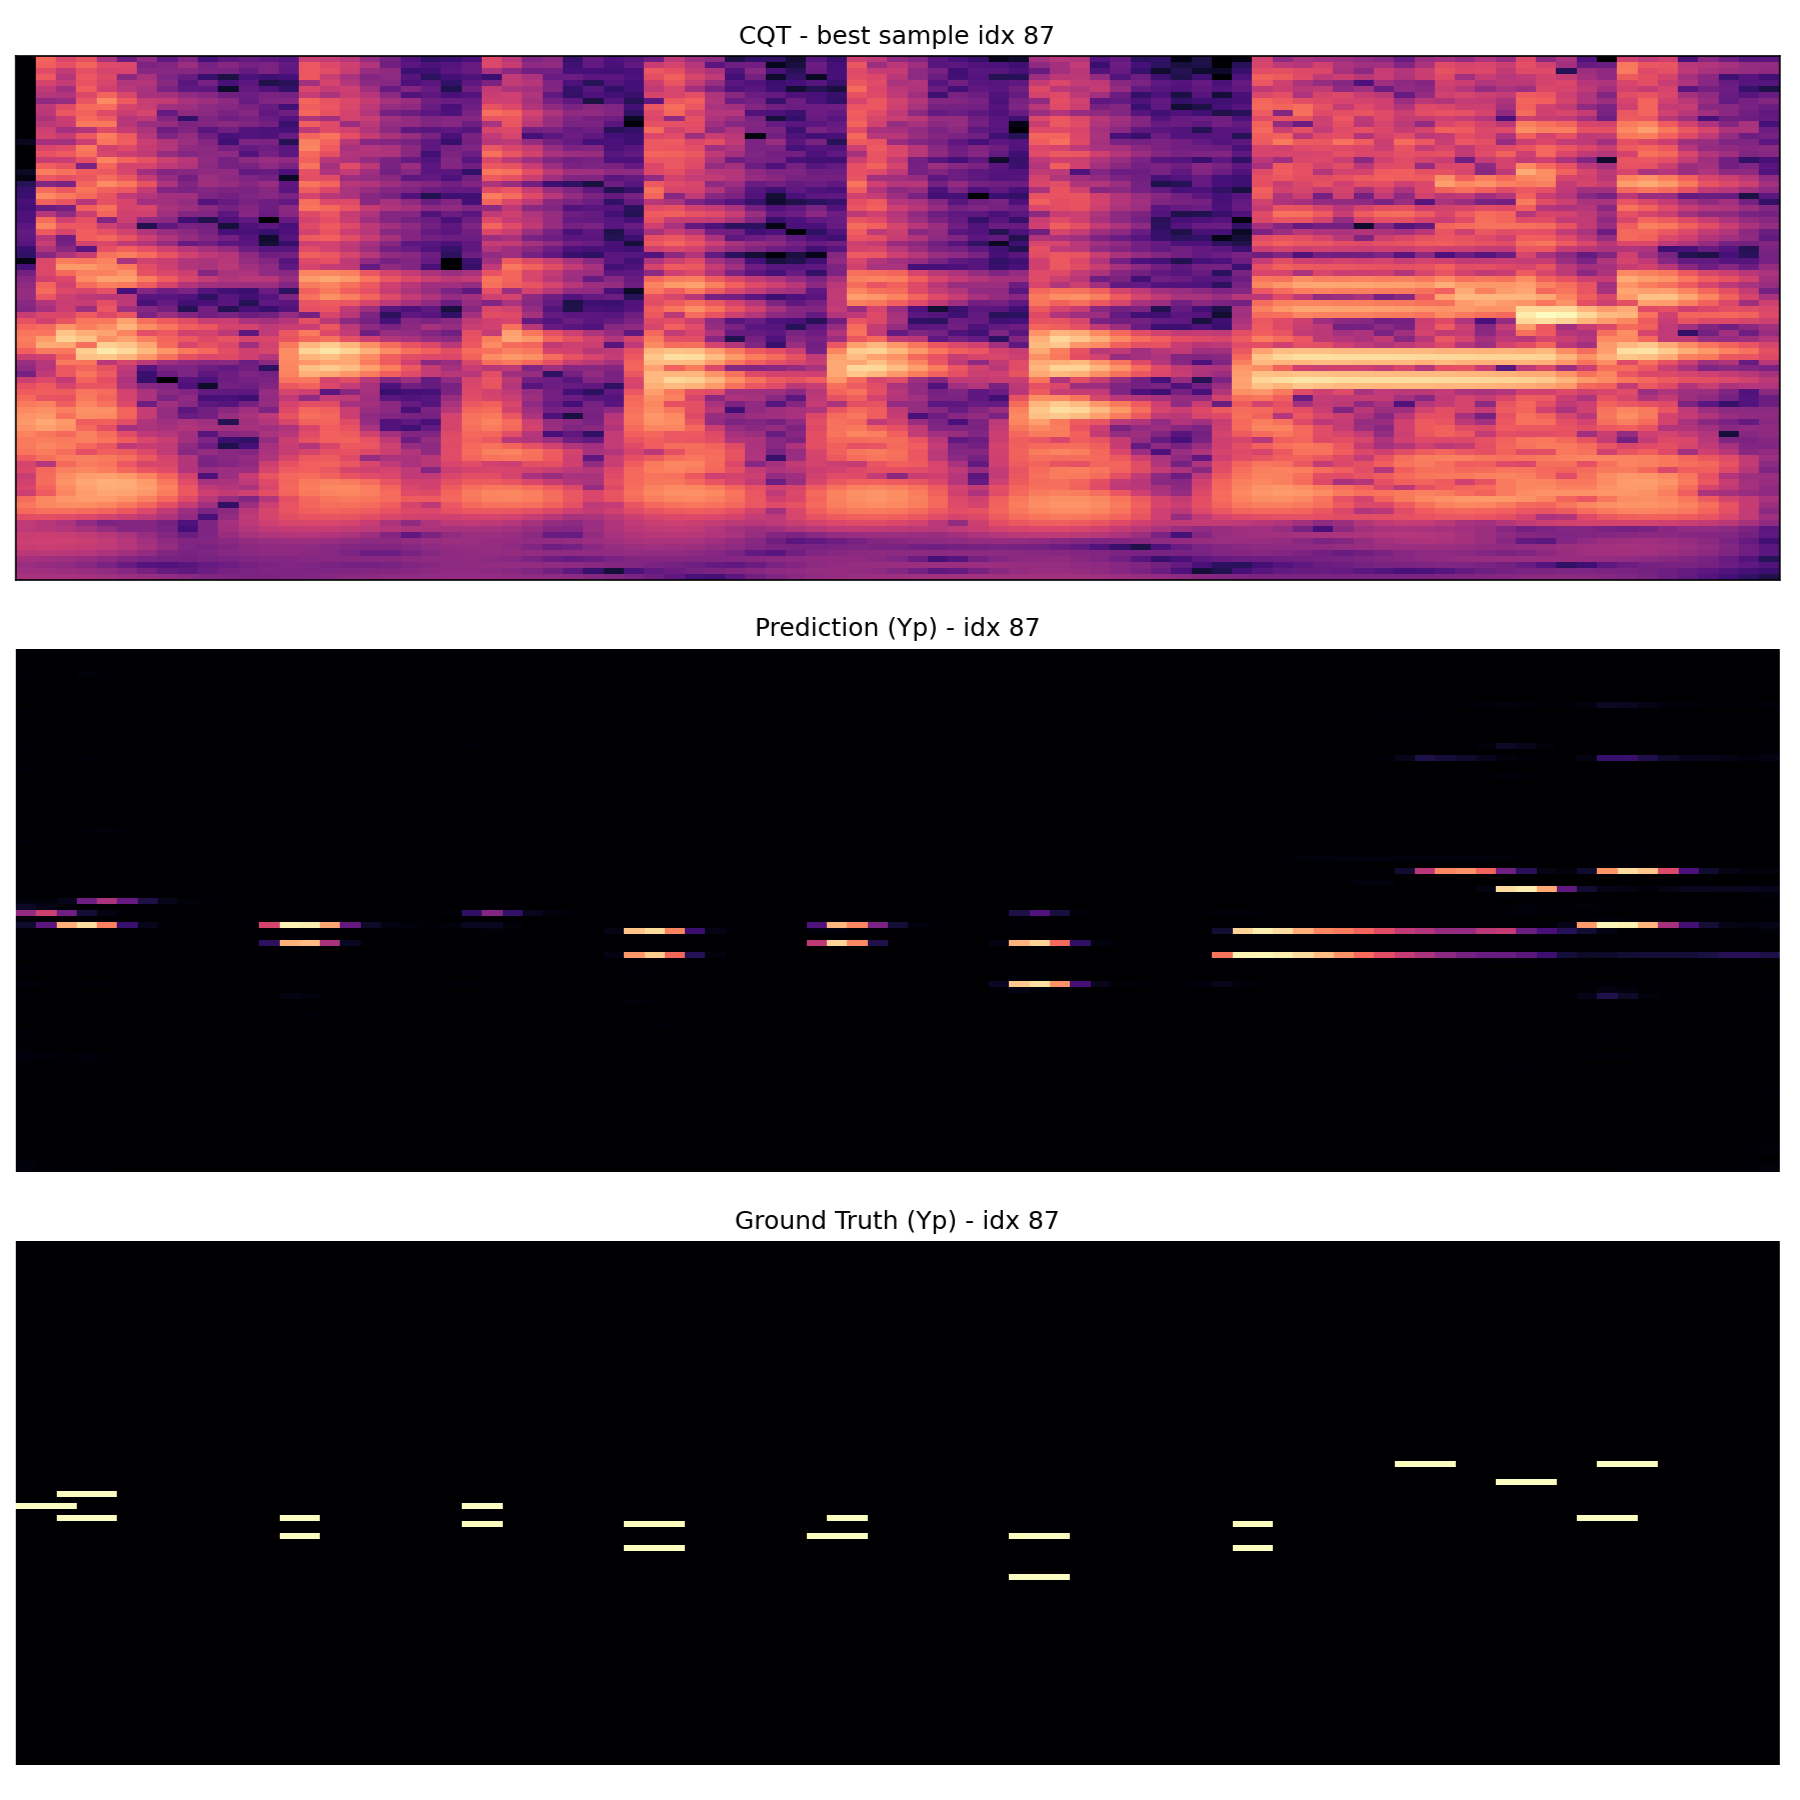
\includegraphics[width=0.9\linewidth]{images/best__87.png}
\end{center}
  \caption{Sample of a well done model prediction}\label{fig:best}
\end{figure}%

\begin{figure}[ht]
\begin{center}
  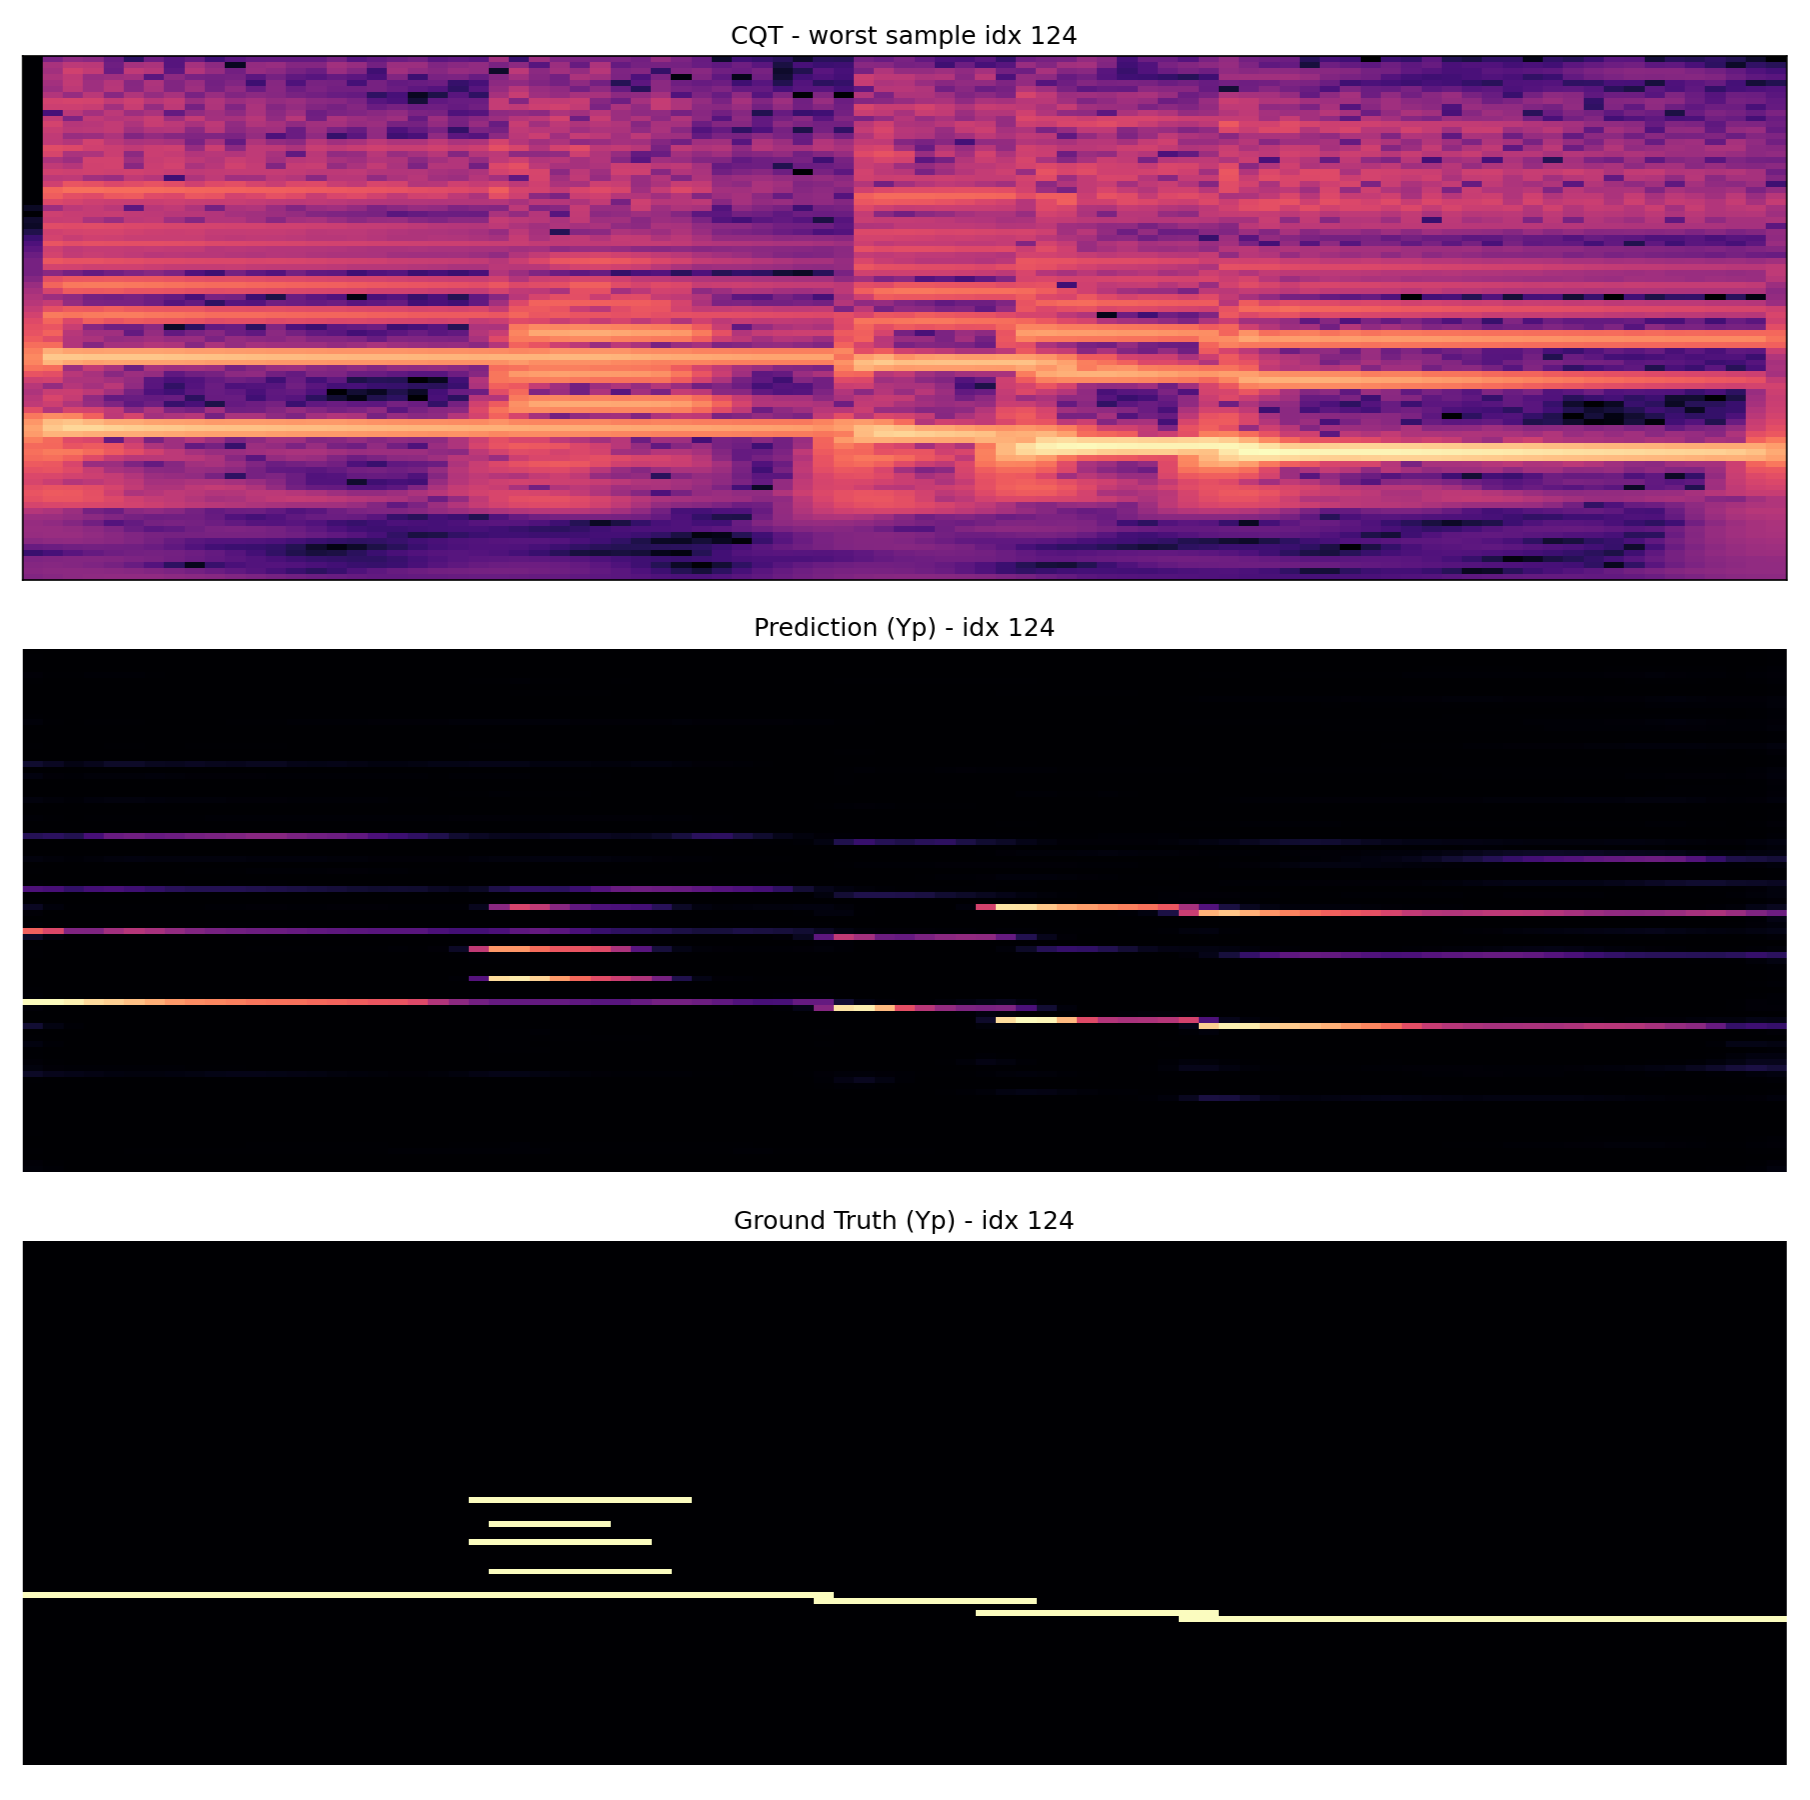
\includegraphics[width=0.9\linewidth]{images/worst__124.png}
\end{center}
  \caption{Sample of a badly done model prediction}\label{fig:worst}
\end{figure}

\section{Conclusions}\label{sec:conclusions}

In this work, we developed a neural network based on two-dimensional convolutional layers for the automatic transcription of audio tracks into MIDI format. The model takes inspiration from the \textbf{\textit{Spotify’s Basic Pitch}}, but was adapted to different libraries and to a custom data-loading pipeline.

Experimental results show relatively low values for precision, recall, and F1-score. However, these metrics proved to be overly strict with respect to the actual application: listening to the generated MIDI files demonstrates that the model is generally effective in preserving the melody and correctly identifying most of the notes, albeit with some imperfections.

The main limitations arise in complex passages, particularly when multiple notes are played simultaneously over longer durations.

It is worth noting that the original Spotify implementation achieves slightly better performance thanks to the use of highly optimized, dedicated libraries. In our case, however, we deliberately re-implemented several steps from scratch, prioritizing the academic value of the project and a deeper understanding of the underlying processes over the use of black-box functions.\\

In summary, the model can be compared to a young pianist who has already developed good skills but still occasionally misses notes when performing more challenging pieces.


\section{Future work}\label{sec:future}

\subsection{Other models: RNNs}

Even if we could train a model with \num{100}\% accuracy on predicting the notes correctly, our approach would still have two intrinsic flaws:
\begin{itemize}
    \item It does not have knowledge about the emphasis with which each note is played: notes played by smashing the piano key or just touching it would be described in the MIDI with the same, arbitrary and constant force.
    \item It has no way to predict control messages, that would be able to deeply change the audio output, without affecting the notes.
\end{itemize}

This led us to think about the intrinsic sequentiality of both the audio (succession of regular samples) and the MIDI (ordered list of messages).
We therefore developed a many-to-many RNN, composed of an encoder and a series of decoders (Figure~\ref{fig:rnn}).
The encoder received in input the audio as sequence of samples, and encoded it into a hidden vector in a latent space.
This hidden vector was then used as input of \textit{(a)} two linear layers, that computed the number of messages and ticks per beat of the song, and \textit{(b)} a RNN decoder, that translated it into the \texttt{numpy} representation of the MIDI.

With this new model, a loss was defined by comparing the expected MIDI with the output, and checking how far each (meaningful) value was from the ground truth.

\begin{figure}[ht]
\begin{center}
   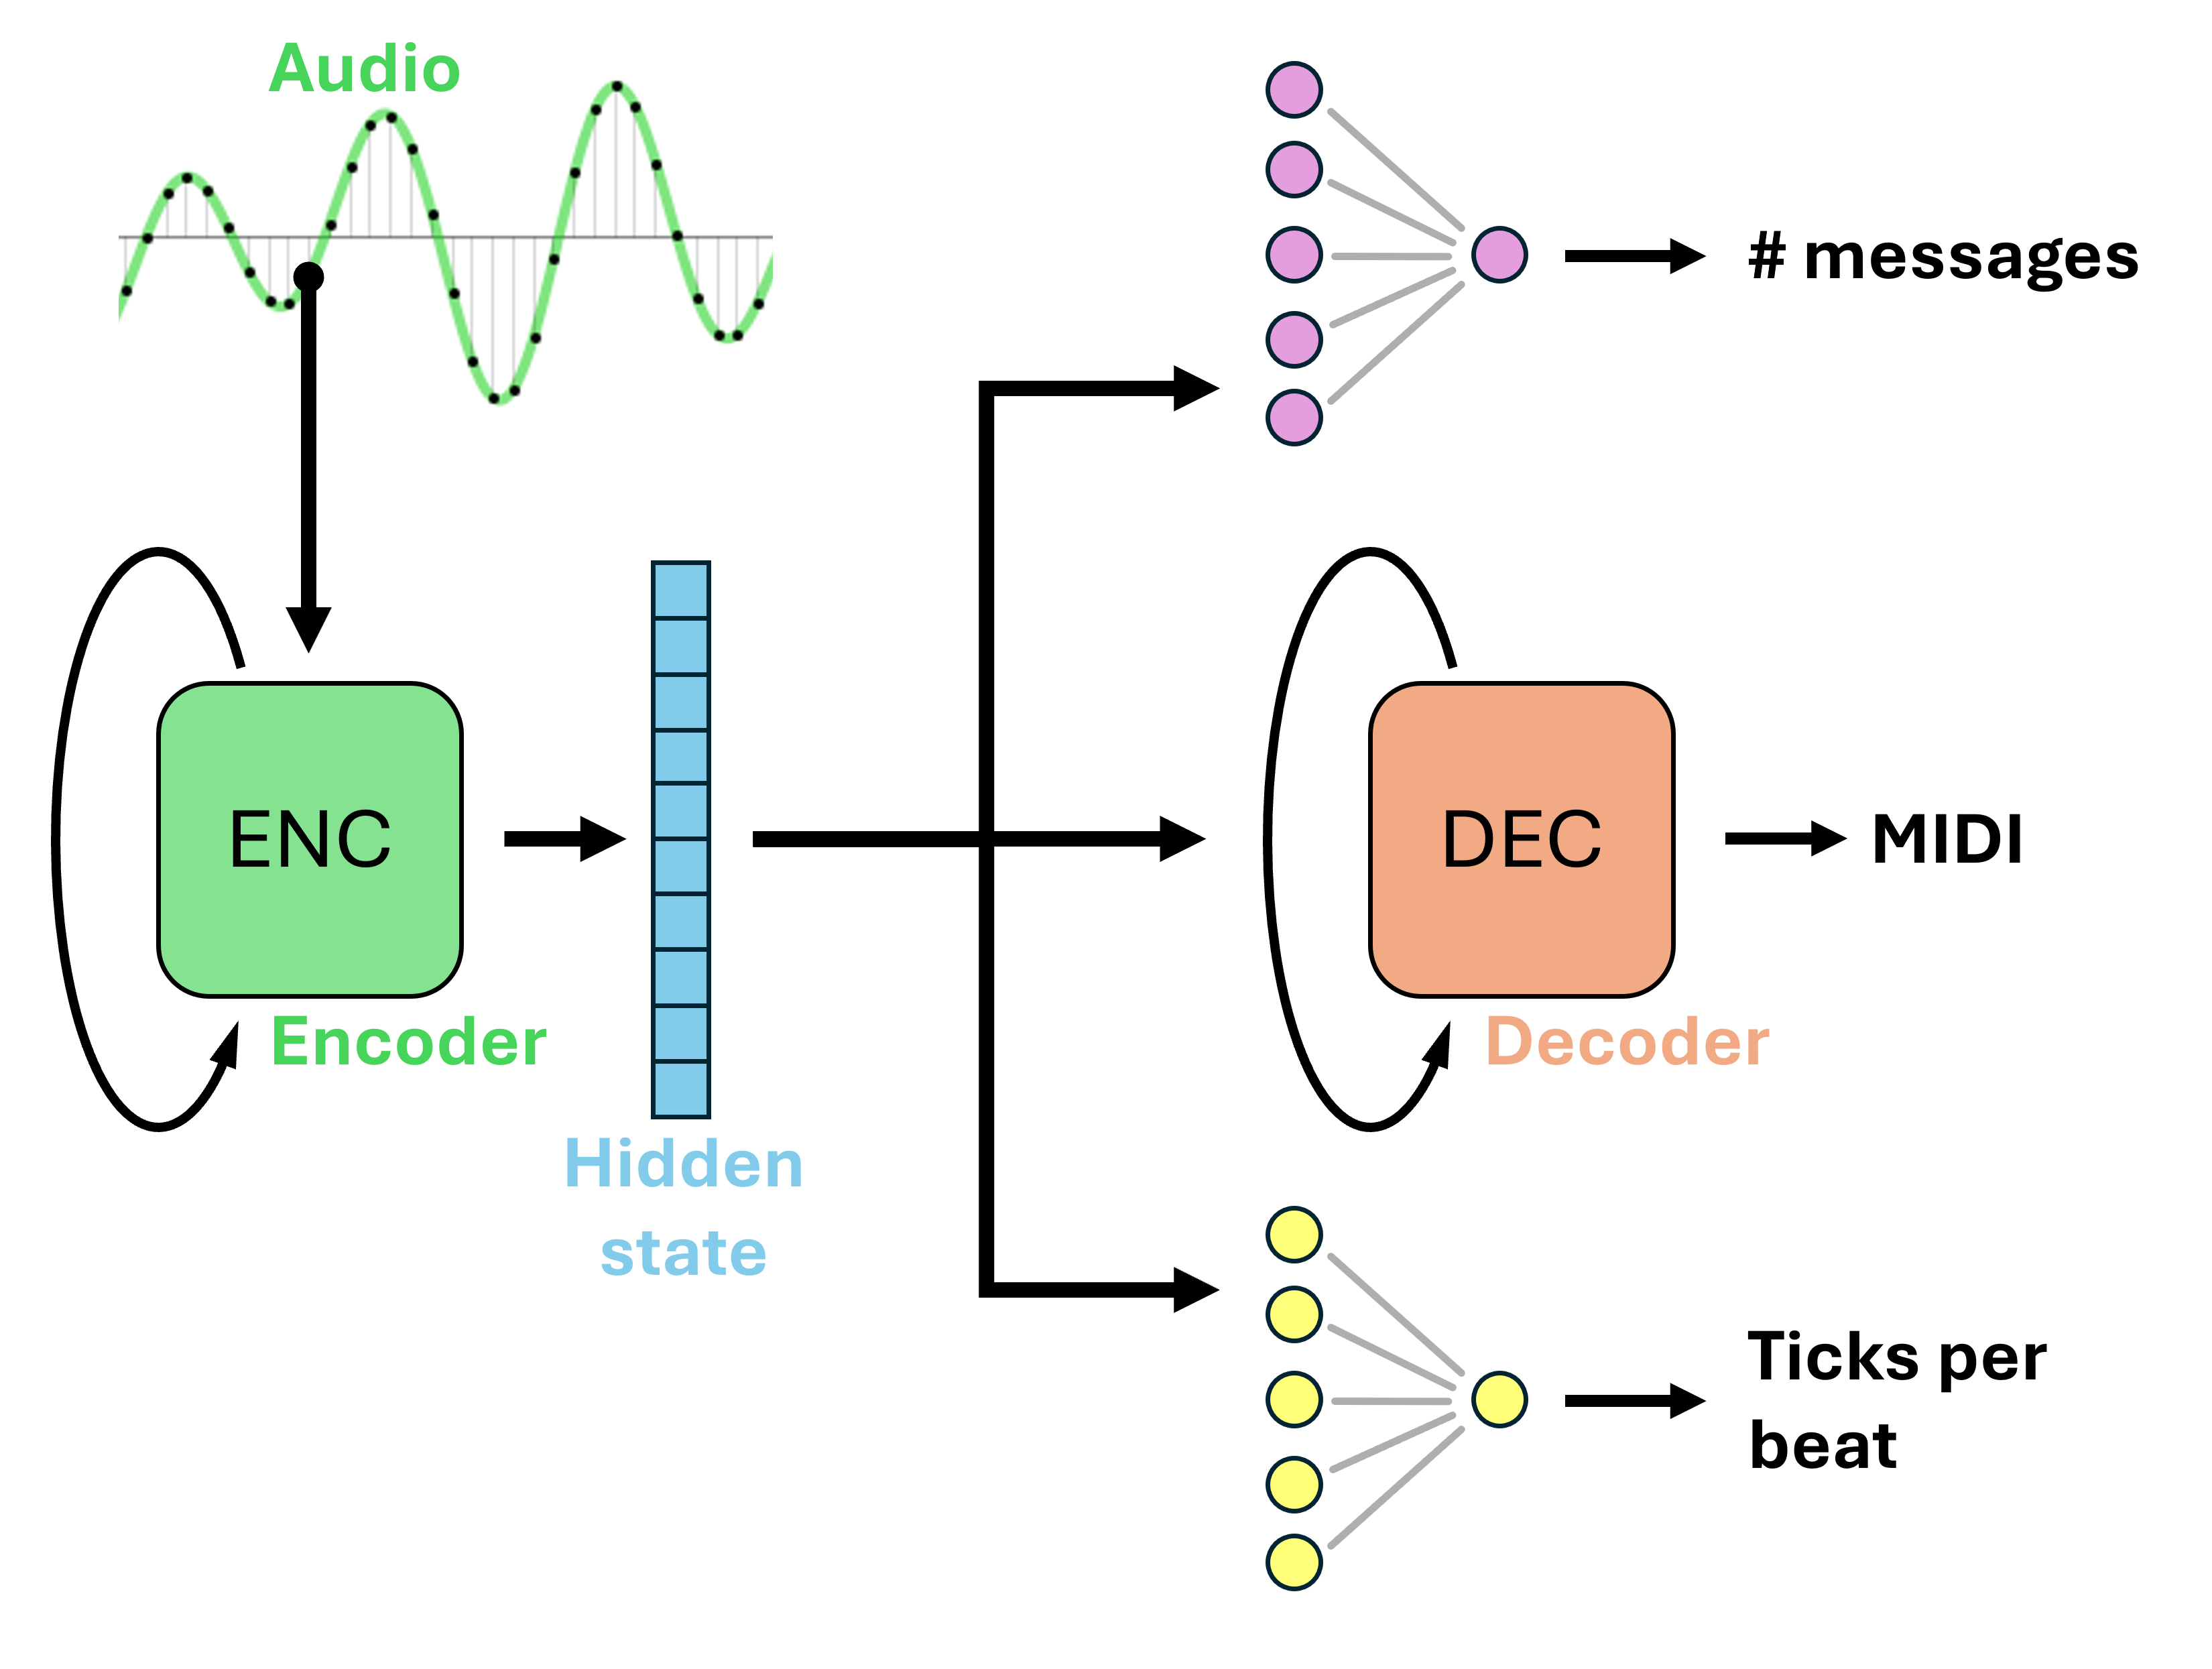
\includegraphics[width=0.8\linewidth]{images/RNN schema.png}
\end{center}
   \caption{The architecture of our RNN.}\label{fig:rnn}
\end{figure}

This model would be able to solve the two intrinsic problems of our CNN:
\begin{itemize}
    \item Each message is predicted as a 6-tuple of floats, that can be interpreted differently for each type of message (which is one of the \num{6} values). This enables the model to also have control on the strength of each note being played.
    \item Control messages are ``just normal messages'' for this model, therefore it should learn how to use them correctly.
\end{itemize}
We believe that the hidden size of this model should be quite large, since it had to memorize everything needed for reconstructing the song.
As such, we elected to have a hidden size of $\num{10000}$.
This meant that the full model would have almost $\num{1000000000}$ parameters, while the CNN only had around $\num{20000}$.
As a consequence of this, the RNN training was extremely long and costly, prompting us to drop the task of training it, settling on the CNN model.

\subsection{Different audio fonts}

As explained in section~\ref{sec:dataset}, the inputs of the network were obtained by rendering the ground truth MIDIs to audio.
In order to do so, we downloaded an audio font representing a piano, and we used it for all the renders.

In retrospect, this was a quite big simplification, that meant that the model specialized in understanding the specific CQT of that particular piano.
We only noticed this when testing the model with ``random audios'' found on the Internet: the performance was on average worse than expected.
To investigate this, we tried rendering a MIDI file with both our usual audio font, and another audio font.
When processing the two audios with our model, the difference was noticeable: the result was considerably better with the usual audio font than with the new one.
Something that could therefore be improved would be having also a dataset of audio fonts, and render each training audio with a random font.

{\small
\nocite*
% \bibliographystyle{ieee_fullname}
\bibliographystyle{plainurl}
\bibliography{egbib}
}

\end{document}
